\documentclass[a4paper,10pt]{article}
\usepackage[utf8]{inputenc}
\usepackage[english]{babel}
\usepackage{indentfirst}
\usepackage{listings}
\usepackage{graphicx}
\usepackage{blindtext}
\usepackage{longtable}
\usepackage{enumitem}
\usepackage{hyperref}
\usepackage{colortbl}
\usepackage{color}
\usepackage[top=2.5cm,bottom=2.5cm,left=2.5cm,right=2.5cm]{geometry}
\pagestyle{headings}
\title{Ftp server in a data diode}
\author{Rusu George, Boulif Ilias, Orinx Cédric}
\date{\today}

\begin{document}
\maketitle
\newpage
\tableofcontents
\newpage
\section{Concept of operations}
\subsection{Introduction to the problem}
Our client would want to prevent his research and development labs against industrial espionage and confidential information leaking. He wants to divide the company network in order to maintain the labs in an isolated environment. Thus, the critical data could not leave the company using the network. But how to be able to transfer files or to assure that all the operating systems are up-to-date? This could be achieved using manual operations where an employee would manually copy the files or the updates on a mass-storage device\footnote{A USB-key for instance.} and then used them or install them on every node from the isolated network. However, this is not the most optimized way and for sure it is not cost less and timeless for the company, without mentioning that there could be dependency problems for applications or updates. This method is also prone to human errors and this could generate security vulnerabilities.

\subsection{Our solution}
In order to address this problem we are going to implement a data diode. In electronics, a diode is a component which conducts the current in one direction. Thus the term of data diode is a set of components that only let the data to travel in an unidirectional way. An example of use case is illustrated in Figure \ref{fig:datadiode}, letting the data pass from a low risk LAN to a high risk LAN but not the way around.

\begin{figure}
\centering
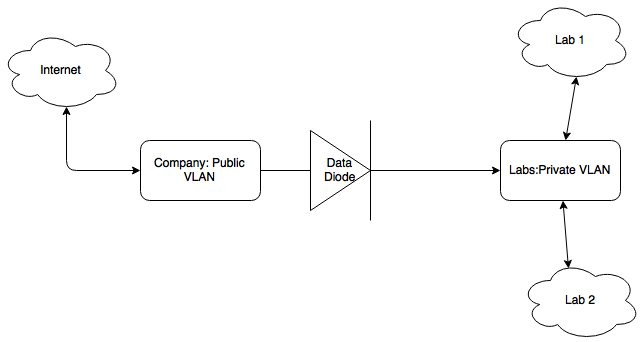
\includegraphics[scale=0.45]{images/dataDiode.png}
\caption{The schema of the usage of a data diode in a company network.}
\label{fig:datadiode}
\end{figure}

A data diode is made using one transmitter(Tx) and one receiver(Rx) both linked using only one fiber cable. Thus, when a digital data is sent through, every bit will be converted\footnote{Using a Digital-to-analog converter (DAC).} into an electrical pulse which will be convert in light pulse using a LED\footnote{Light Emitting Diode.}. Then, the output light will pass through the fiber cable and as soon as the photons are reaching the receiver, they will be converted firstly into an electrical pulse by a photo diode and then in bits\footnote{Using an analog to digital converter (ADC).}. Since there is only one fiber, data can only travel in one way.

One major problem of this system is the network transport protocols(layer 4 in the OSI model) that applications are using. The most used transportation protocol nowadays is TCP. However, TCP is a bi-directional protocol which need the 3 way handshake in order to start a connection, thus there must be at least two fiber cables. In contradiction, UDP does not require a handshake process because it does not provide reliability, ordering, data integrity and does not set up a dedicated end-to-end connection automatically. Thus, UDP protocol does not necessarily require a bi-directional data transfer. Therefore, the use of such a protocol is recommended when dealing with applications that are not sensitive to data loss or that implements an error checking system. Hence, the use of the UDP protocol within the data diode.

It seems obvious now that the transport protocol used between the transmitter and the receiver of the data diode is UDP. However, this brings multiple problems. One of the problems is how to be able to use applications that requires TCP. Another problem could be the reliability of the digital data transfer in the data diode, how can we ensure that there will not be any data loss during the transfer. We will address to those questions further down in this document.\bigskip

Furthermore, system administrators would dispose of a file transmission mechanism from the low level to the high level in order to maintain all the computers up to date. This will be done using the FTP protocol and will be explained in the next section.

\subsection{Our System description}
The data diode concept is a well orchestrated combination between hardware and software. The data diode is composed of two servers: a transmitter and a receiver. We could consider that the transmitter server is connected to the low security risk LAN where a connection to the internet is made and where all the employees are connected. The receiver is connected to the high security risk LAN where all the labs are connected and where critical informations are stored.

The transmission of the information will be from the low side to the high side and blocked the way around as shown in Figure \ref{fig:UDPDD}.

\begin{figure}
\centering
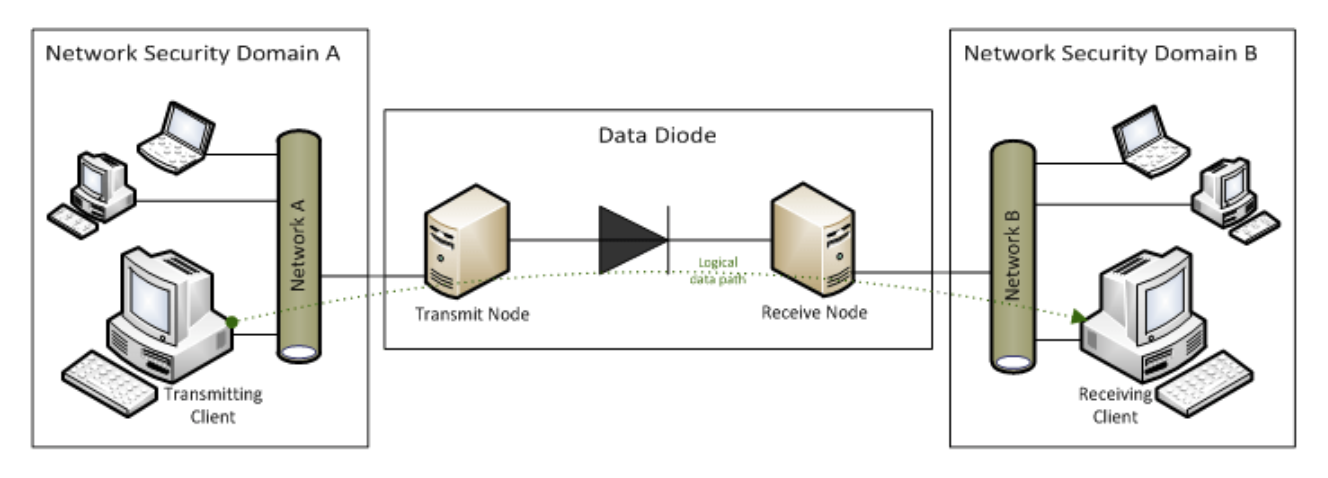
\includegraphics[scale=0.5]{images/logical-scheme-DD.png}
\caption{Data logical path within the data diode.}
\label{fig:UDPDD}
\end{figure}

\subsubsection{Hardware}
The following table presents the components used for the data diode implementation. We should mention that both transmitter and receiver possess two NICs\footnote{Network interface controller.}: one for the communication within the LAN and one for the data diode.\bigskip
\begin{table}[!h]
\centering
\begin{tabular}{|p{3cm}|p{10.5cm}|}
	\hline
	\textbf{Components} & \textbf{Description}                 \\
	\hline
	Transmitter server  &  a physical machine or a virtual machine. The NIC for the data diode will be set in transmission mode only. \\
	\hline
	Receiver server  &  a physical machine or a virtual machine. Similar to the transmission, the NIC will only be set in a receiver mode.\\
	\hline
	One fiber cable & This optical fiber allows communication between the low server and the high server.\\
	\hline
	Two fiber NIC and two UTP/RJ45 NIC & On each side, there will be one fiber NIC for the data diode and one UTP/RJ45 NIC for the communication in the LAN.  \\
	\hline
\end{tabular}
\caption{Components description}
\label{tab:component}
\end{table}
\subsubsection{Software}
The Linux distribution which will be used in our project will be Ubuntu 16.04 LTS. We will have two linux machines, one on the transmitter side and one on the receiver side. 

The data diode will be easily administrated using a web interface running on a Django server. The web interfaces will be hosted on both servers according to the server location in the company network (transmission interface on the transmitter server, same for the reception interface). It will be described in more details further in this document.

Every configuration script used by the web interfaces will be a combination of Python language and Bash language.
\subsubsection{First overview on the project implementation}

Let's start by explaining which protocol shall be used in the data diode. Remember that our main goal is to create an isolated environment but also to facilitate the file transfer process to the high security zone. As we mentioned earlier, we are going to use the FTP\footnote{File transfer protocol.} protocol. There are some alternatives to FTP such as BlindFTP, SFTP, etc. However FTP and SFTP are using TCP as their transportation layer protocol. Thus, we are going to use between the transmitter and the receiver the BlindFTP which use UDP instead.

BlindFTP is a simple Python script which was especially created for the communication between the two servers over an unidirectional network. It is simply a tool for transferring files from one side to the other. Despite the fact that it uses UDP, there is no acknowledgement of received packets but this is compensated by a redundancy of the data. Another advantage is the language used, as it is written in Python the result code is relatively simple and very portable to Windows, Linux or MacOS.

It is now time to have a look at our entire system, let's have a look in Figure \ref{fig:sysschem}.\bigskip

\begin{figure}
\centering
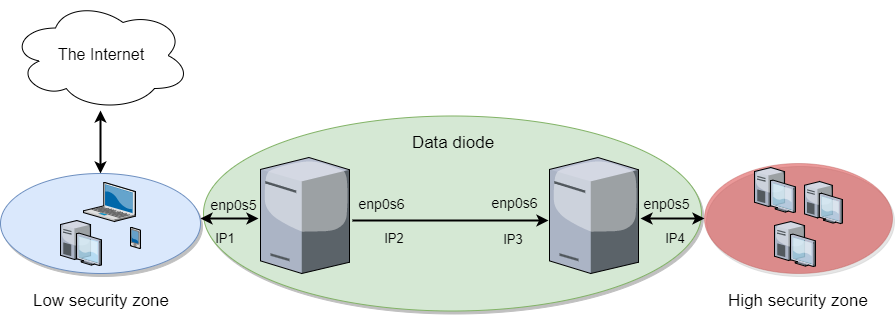
\includegraphics[scale=0.5]{images/DataDiodeSchema.png}
\caption{Entire system.}
\label{fig:sysschem}
\end{figure}

We should note that between the transmitter and the other peers a TCP connection can be used to communicate (transmitter web interface). And this is the same for the receiver, after the data goes out from the network diode the transportation protocol could be TCP with other computers (receiver web interface) . In this way, we are not dealing anymore with the problem of application transportation layer. 

\subsection{Users} 
In general every employee of a company has a unique ID, a grade, a job title and so on. The company owner or the manager in charge with the security could choose which grade or which person can have access to the administration web interface, of course this exclude the systems administrators. Every user information is managed and stored by the company in their own databases and this is a requirement for the working of the data diode. Despite that, this is out of our scope, we will assume that our client has his own user database and we will consider two types of users to make our explanation simpler : the \textit{administrators} and all others \textit{users}.

A \textit{user} is simply an employee of the company. Every employee has limited access into the company's files according to their job title or to the specific rule defined by their supervisor.

An \textit{administrator} is a user in charge of operating and maintaining the data diode. It is the only authorized person to configure or maintain the well operating of the data diode and this is mandatory. He will have to know how the data diode is working, should know how to interact with it using the web interfaces, but mostly he should be able to reconfigure it or restore it as quickly as possible in case of a security breach or a system failure. We should not forget to mention that an administrator should not have access to some strict secret files of the company but only to IT department files.


\subsection{User Interface}

As we mentioned earlier, the administration of our data diode will happen through a web interface. There will be one web interface hosted on the transmitter which will allow to transmit files or update packages from the lower network to the higher network. But, on the other hand, there will also be a receiver web interface for each user to manipulate his transferred data more easily.

Each user should log in from both side to use the platform. Here is an overview of our log in page:

\begin{figure}[!h]
\centering
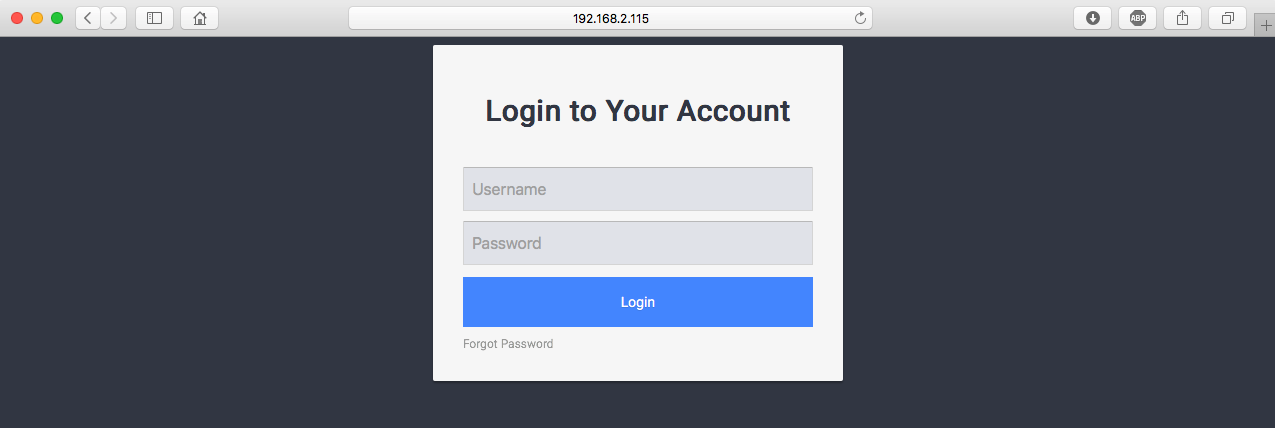
\includegraphics[scale=0.35]{images/login.png}
\caption{Login page.}
\label{fig:logpage}
\end{figure}

Once login is made, the user will be prompted to the web interface of the transmitter or the receiver. The page are shown in Figure \ref{fig:transuserpage} and Figure \ref{fig:receiveruserpage}.


\begin{figure}[!h]
\centering
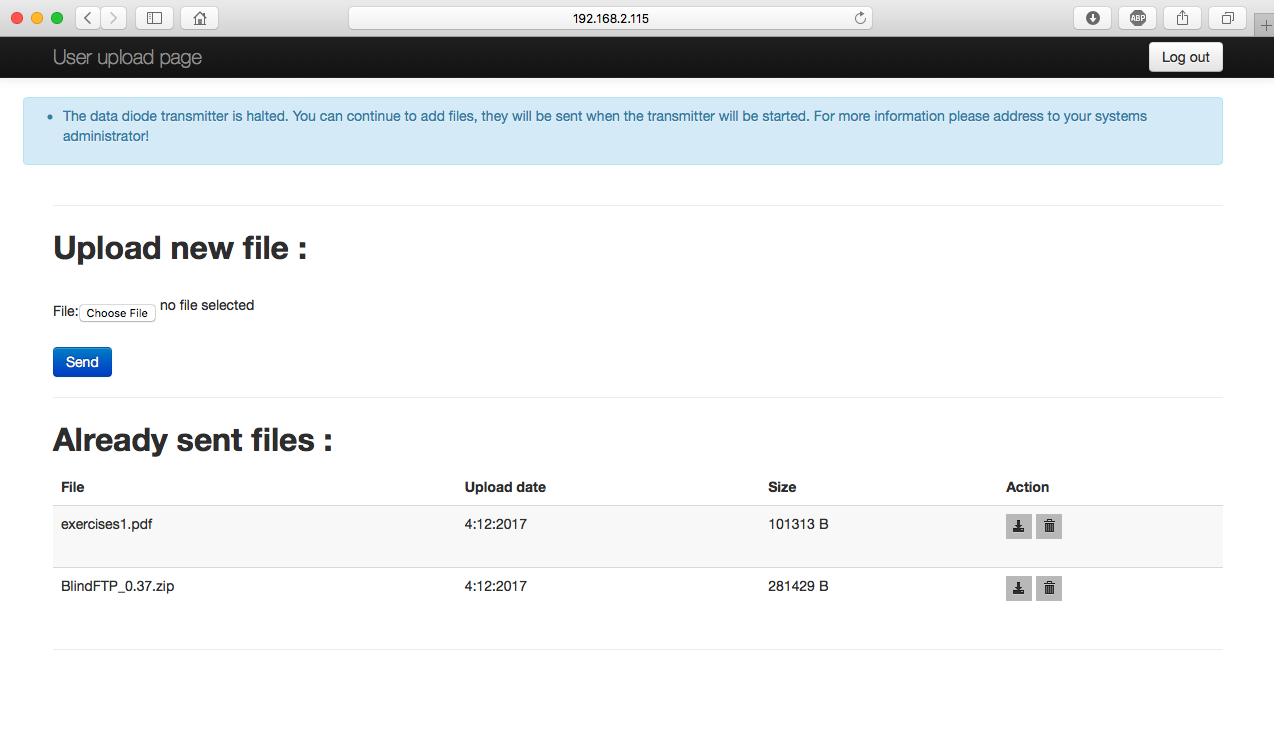
\includegraphics[scale=0.35]{images/usertransmitter.png}
\caption{Transmitter user page.}
\label{fig:transuserpage}
\end{figure}

\begin{figure}[!h]
\centering
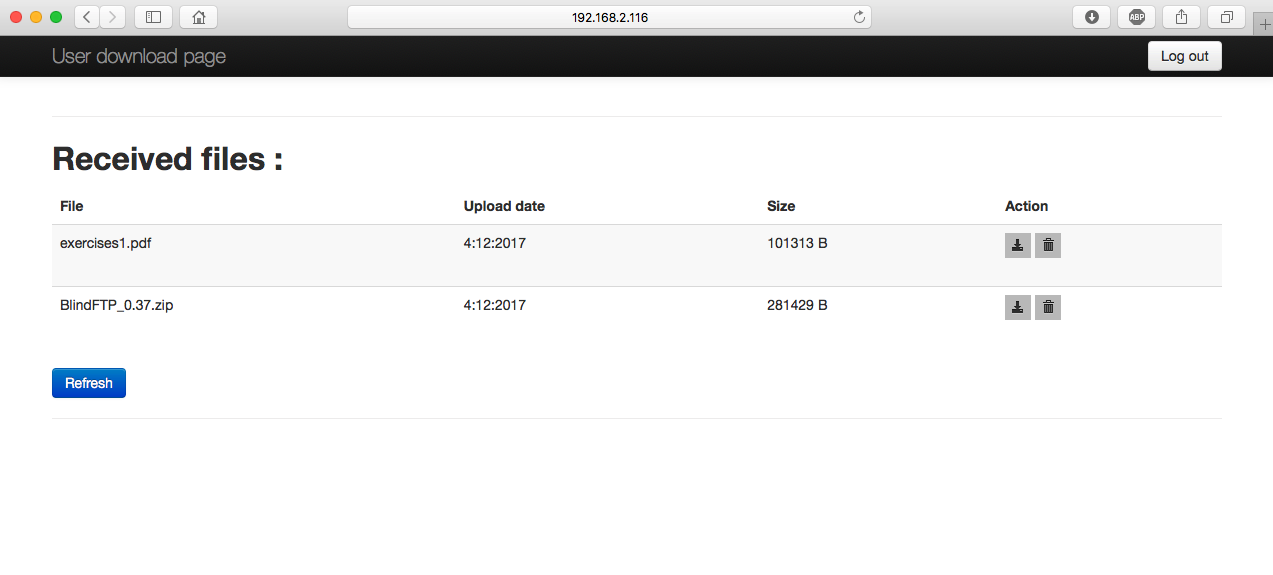
\includegraphics[scale=0.35]{images/userreceiver.png}
\caption{Receiver user page.}
\label{fig:receiveruserpage}
\end{figure}

On the other hand, an administrator can transfer files or he can upload an update package from his own computer. The admin. interface is shown in Figure \ref{fig:transadminpage}
and in Figure \ref{fig:receiveradminpage}.
\begin{figure}[!h]
\centering
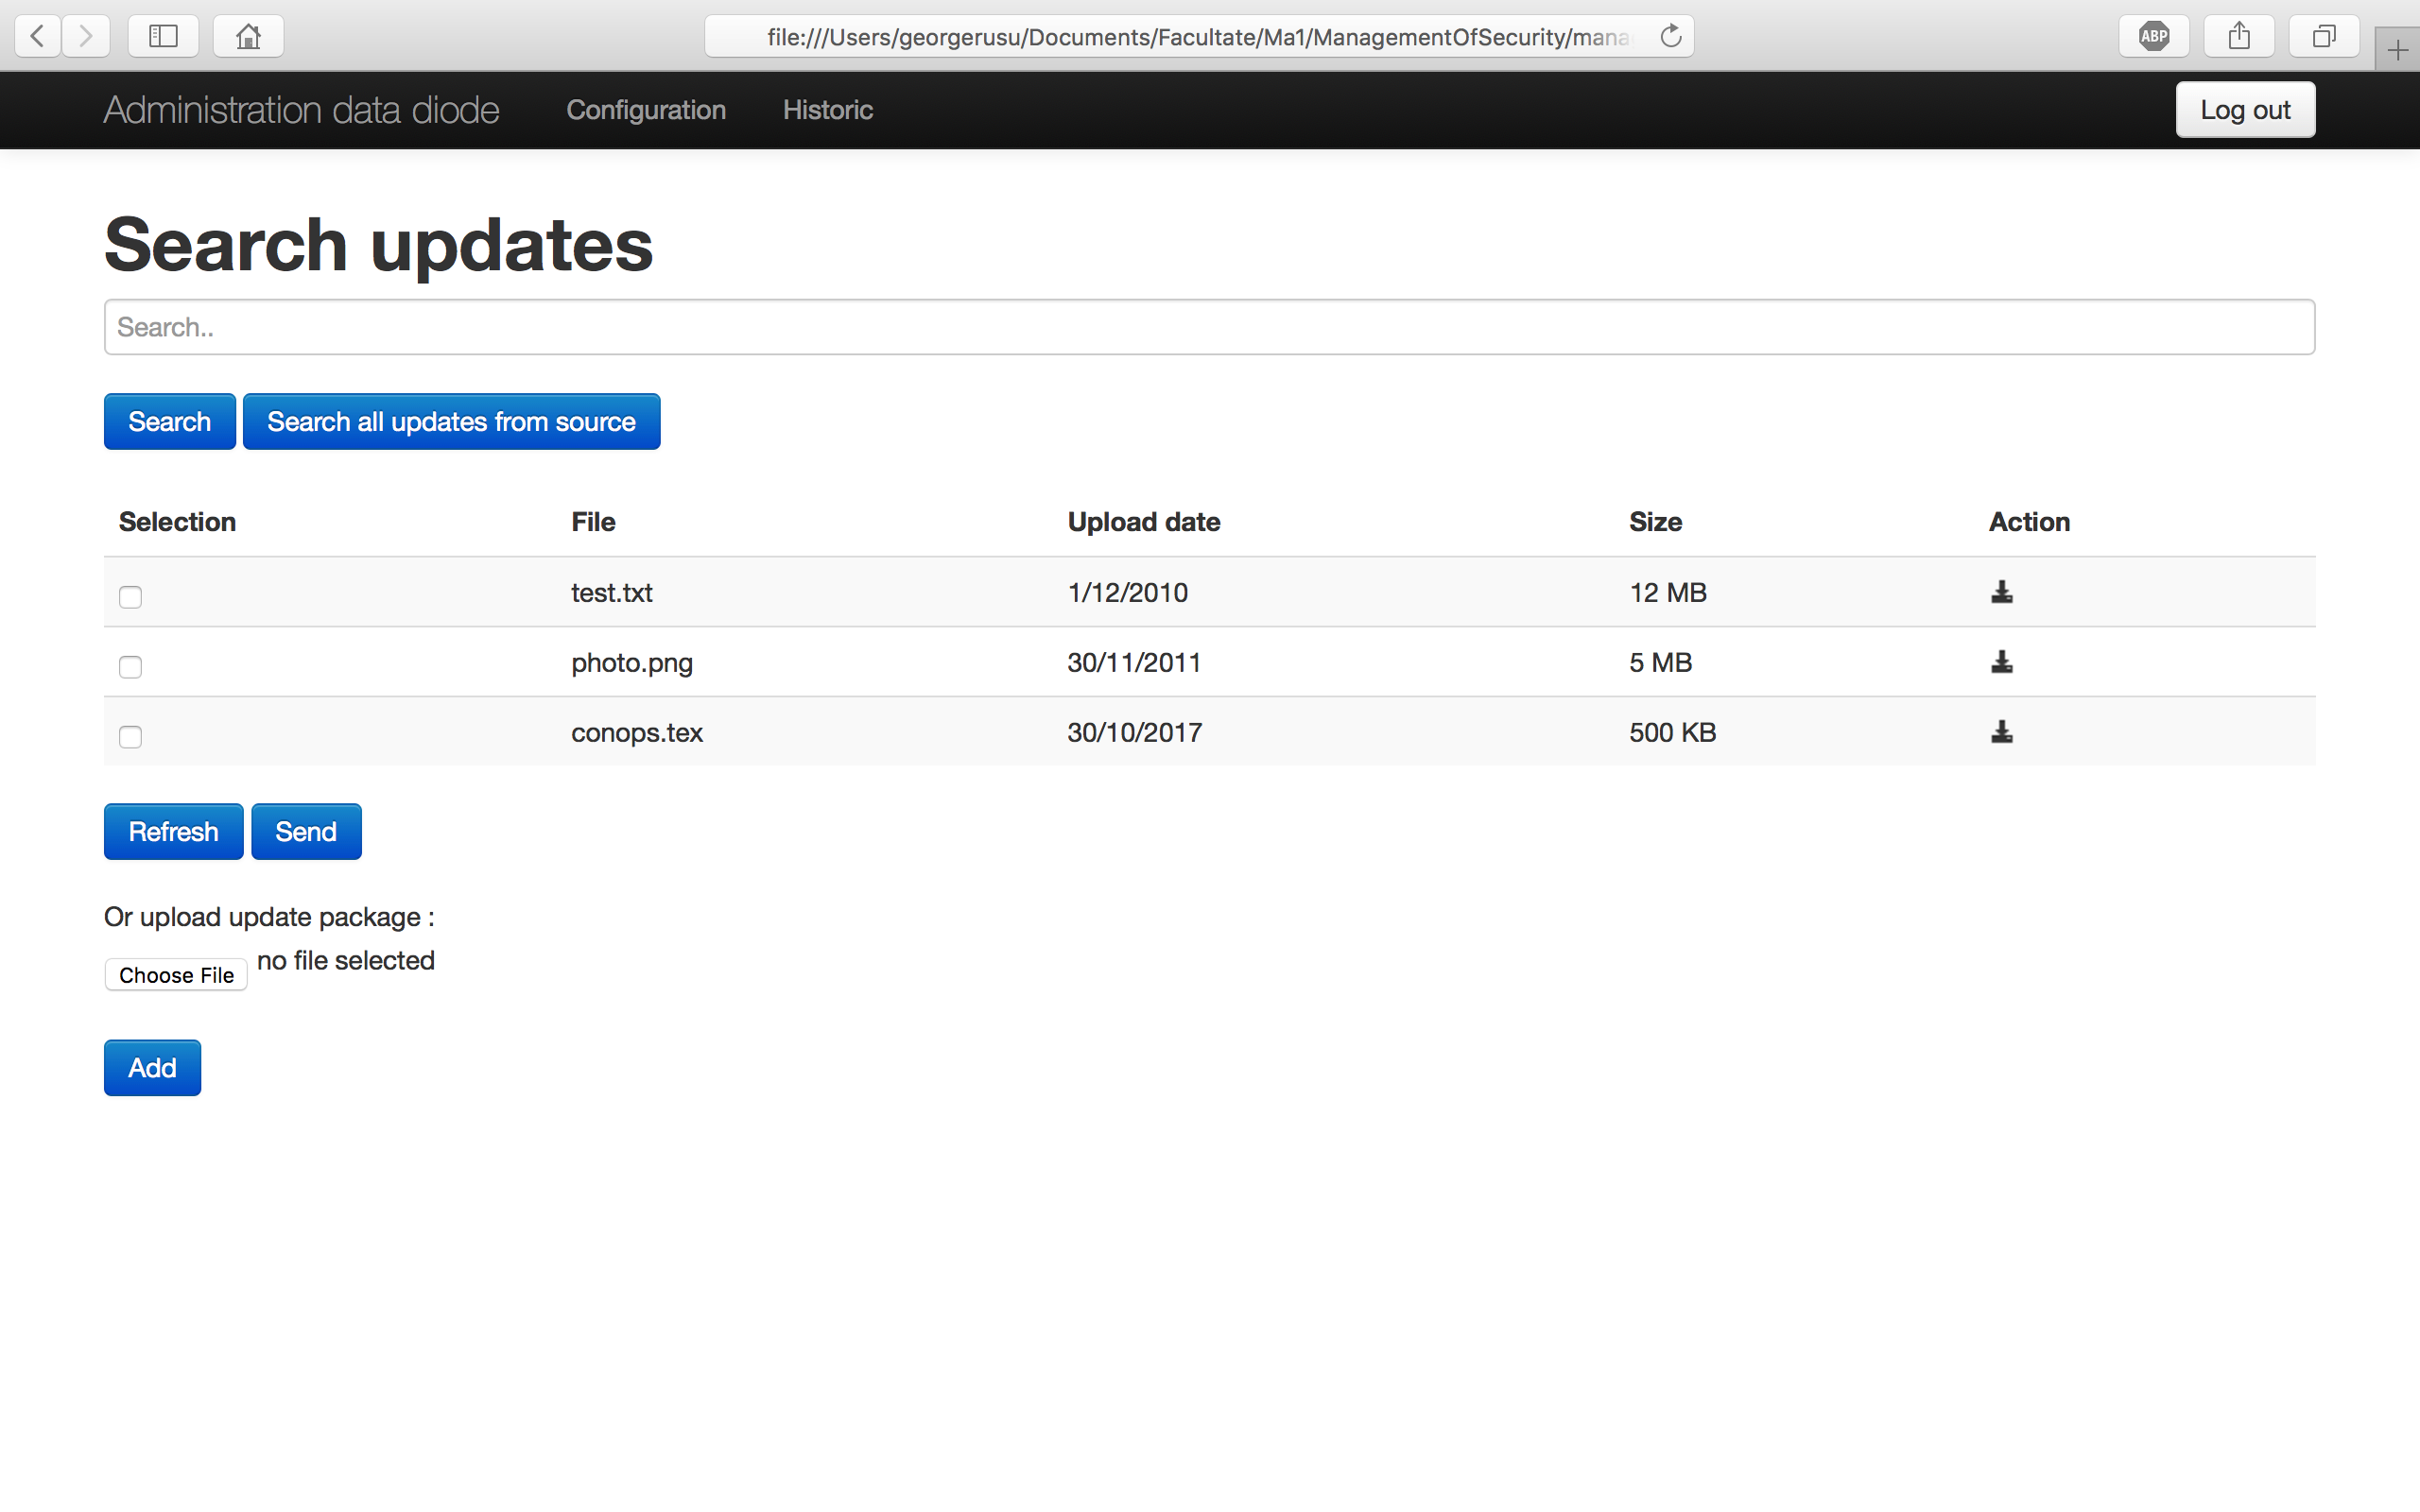
\includegraphics[scale=0.35]{images/admintransmitter.png}
\caption{Transmitter admin page.}
\label{fig:transadminpage}
\end{figure}

\begin{figure}[!h]
\centering
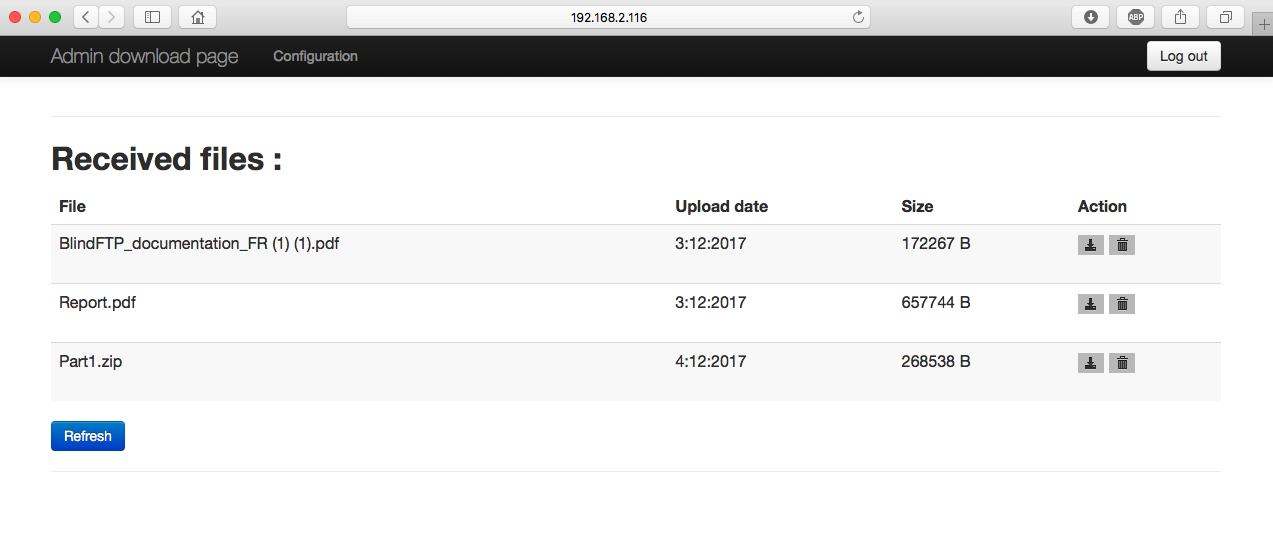
\includegraphics[scale=0.35]{images/adminreceiver.png}
\caption{Receiver admin page.}
\label{fig:receiveradminpage}
\end{figure}
\clearpage
\subsection{Usage of the WEB UI}
In this section we will explain how to use our web interfaces from different point of views.
\subsubsection{General usage}
In both cases, all users have to identify themselves through the login page with their credentials. They must fill in the form with their own username and password (Figure \ref{fig:logpage}). Once the form is submitted, the authentication will bring them respectively to their dedicated page.\bigskip 

In the case of a user connection, he will be redirected to the user transmission page according to his network location: if he is in the low security zone he will be prompted to use the transmission interface (Figure \ref{fig:transuserpage}) or he will get the receiver interface page (Figure \ref{fig:receiveruserpage}) if he stand on the high security zone (after the data diode). 

On the transmission page the user can choose among his own documents a file to send through the data diode by using the \textit{send} button. On the reception page, the user has a list of all the received files which he can refresh, download or delete.\bigskip 

When an administrator will log in, similarly to the user mechanism, he will be redirected according to his network location : on the transmission interface or on the receiver interface, respectively Figure \ref{fig:transadminpage} and Figure \ref{fig:receiveradminpage}.

On the transmission page, in addition to a simple user, the administrator has the power to configure the data diode, this will be presented later in this document.

On the reception page, the administrator has access to only his transferred files through the data diode. In this way, we are sure that the confidentiality is preserved by the administrator.  

If an administrator wants to maintain (updates) the company's computers he could download on his machine the needed update packages and transfer them easily to the high security zone. All this is made possible thanks to our interface and file transfer system. He can then update all the machines using some Linux script or to use the web interface to download each update package manually on the desired machine. Of course the latter method is not the most optimal, but it could serve in case of a need for a system downgrade or an application downgrade on a workstation. 


\subsubsection{A Technical file transfer usage}
We have said earlier that there will be a web interface running on both sides of the data diode. When a user will want to send a file, he would have to first log in. The log in page will use the database of the company in order to authenticate users and to verify each user permissions. However, on the high security zone, the database would not be reachable because of the unidirectional data diode. Thus, once a user would want to send a file to the other side, there will be a daemon which will create a permission and ownership system in order for the other side to recognize to whom the file belongs to:
\begin{enumerate}
\item[-]For \emph{UserX} the folder will be named $\triangleright$ \emph{SHA256(UserX+isAdmin);PBKF2SHA256(password)}.
\item[-]For every \emph{UserX}'s file, it will be copied in the \emph{UserX}'s folder and renamed $\triangleright$ \emph{timestampUpload;filename}.
\end{enumerate}
 
On the other side, there will be of course another receiver daemon which will according to all received folders create the database. Indeed, when the \emph{UserX} has already sent a file, the receiver will get in the receiver folder the corresponding \emph{UserX}'s folder. When the user would want to log in, the daemon will check his credentials with the folder name. If it is a match, then the user \emph{UserX} will be inserted in the receiver database. He will then have access to the web platform and to his sent files. Of course there is also a second daemon which for every user's folder will read and list all the files properly to the user:

\begin{enumerate}

\item[-] The received file \emph{timestampUpload;filename} will be shown to his owner as $\triangleright$ \emph{filename} and with others property such as the size and the date when the file was uploaded into the data diode.
\end{enumerate}

In this way, the main verification will take place on the transmitter side where the database can be accessed : if a user has the permission to transfer a file, he will be able to transfer the file from the transmitter side. Thus, if the file is transmitted to the receiver side, it means that the user has an access granted on the security zone and thus he has already been verified. However, if a user has not yet used the transmission system of the data diode, he will not be able to connect to the interface from the receiver side. Once the user has been added to the security zone database, then the log in process will no longer use the folder checking daemon but instead will query directly the database as usual.

It is very important to mention that employee's name and password will not be shared in clear text, a hash of SHA-256 will be used for the employee's name and the isAdmin property and a PBKF2SHA256 will be used for the password.

\subsubsection{Configuration panel for the admin}
The admin can configure the IP address of both the transmitter and the receiver. In this case, we are not talking about the communication within the data diode but about the communication to other peers of the network. Furthermore, he has the power to configure the data diode : he can start/stop the file transfer protocol and change the transmission/reception folder.

\begin{figure}[!h]
\centering
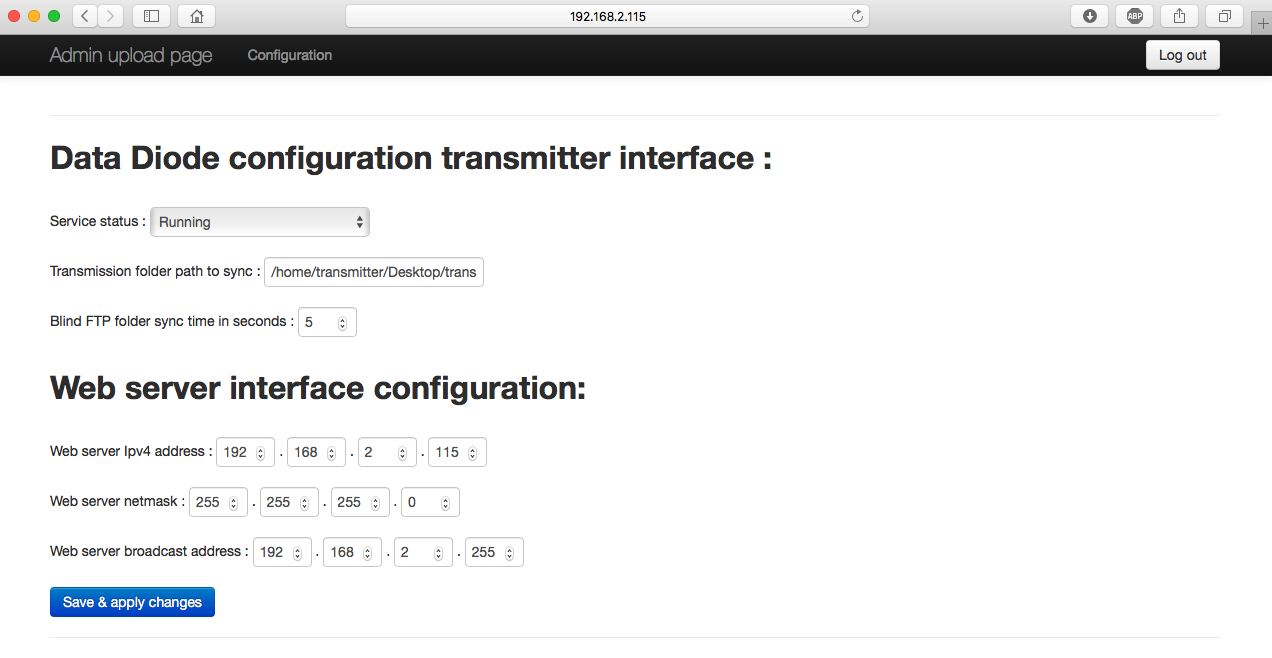
\includegraphics[scale=0.35]{images/admin-configTrans.png}
\caption{Configuration panel for admin on the transmitter side.}
\label{fig:configadminpagetrans}
\end{figure}
\bigskip
\begin{figure}[!h]
\centering
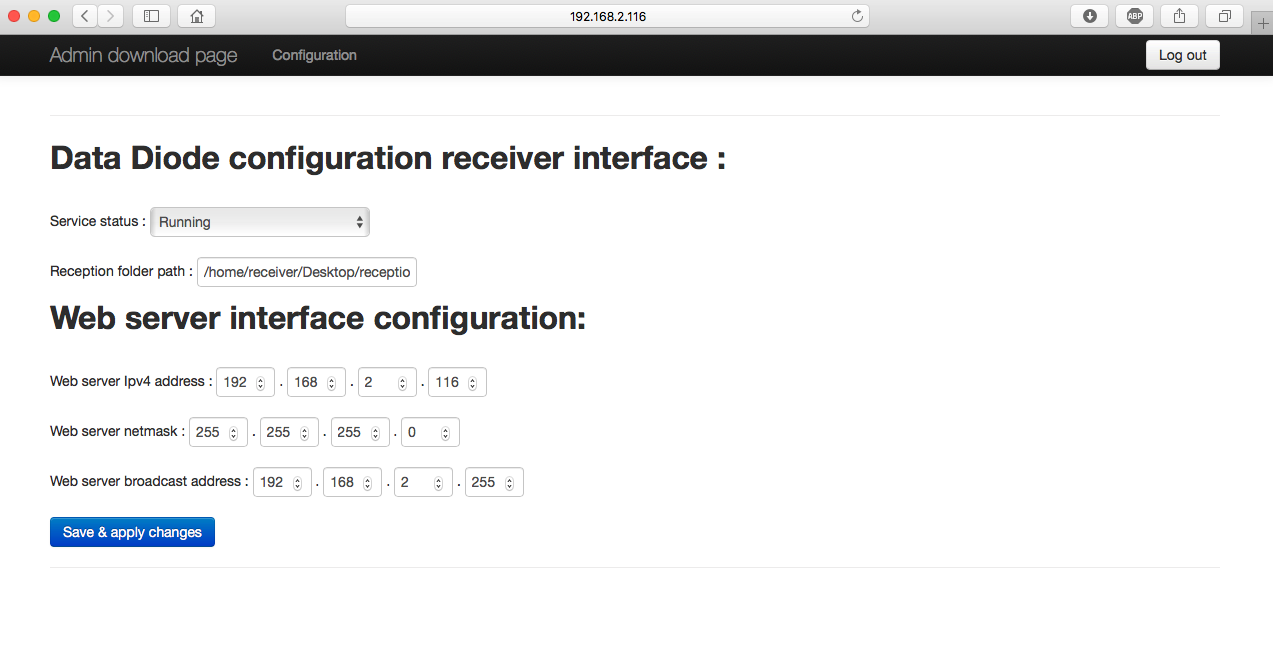
\includegraphics[scale=0.35]{images/admin-configReceiv.png}
\caption{Configuration panel for admin on the receiver side.}
\label{fig:configadminpagereceiv}
\end{figure}

\subsubsection{Installation}
\paragraph{Set up}
The following steps should be followed in order to have a fully operational data diode:


\begin{enumerate}
\item \textbf{Network settings} The administrator has to connect to machines using the following credentials:
	
\begin{enumerate}
\item[-]On the transmission side $\triangleright$ user: transmitter \& password: abbaabba
\item[-]On the receiver side $\triangleright$ user: receiver \& password: abbaabba
\end{enumerate}
 
Once logged in, he should edit the files\footnote{We are assuming that an administrator should be capable of editing the configuration file of a Linux operating system network interfaces.} according to the company's LANs settings. These files are located at:
\begin{enumerate}
\item[-] For the transmission side : \emph{/home/transmitter/Desktop/DataDiodeTransmiter/interfaces}
\item[-] For the receiver side : \emph{/home/receiver/Desktop/DataDiodeReceiver/interfaces}
\end{enumerate}

Both web interface should be now accessible from a browser on port 8080.

\underline{WARNING}: The passwords for both machines should be changed!

\item \textbf{Linking the company database with the transmitter authentication system} The administrator has to edit the file at \emph{/home/transmitter/Desktop/DataDiodeTransmiter/DataDiode/settings.py} and change the database configuration to the company's database configuration. The authentication on the transmitter side should now be operational.

\item \textbf{Enabling \emph{Blindftp} reception on the receiver side} Log in on the receiver side using username: admin \& password: admin and enable \emph{Blindftp} reception service.

\underline{WARNING AT YOUR OWN RISK}: The default account username: admin \& password: admin can be disabled in the file located at \emph{/home/receiver/Desktop/DataDiodeReceiver/DataDiode/settings.py} by changing the \emph{ADMINACCOUNT} attribut to 1 instead of 0. However, after a system restart, the data diode reception should manually be enabled if the receiver database is empty

\underline{WARNING}: The default account will be automatically disabled at first log in.

\underline{NOTE}: The default account has not the power to see sent files.

\item \textbf{Enabling \emph{Blindftp} transmitter on the transmission side} Turn on the transmitter \emph{Blindftp} service and test it by sending a file.

\item \textbf{Checking the receiver side reception} On the reception side, the administrator should now be able to connect using his company credentials and he should have received the sent file.

\end{enumerate}
The data diode should be fully operational. \\  
\underline{BACKUP OF ALL FILES HIGHLY RECOMMENDED}: The administrator should now backup/compress all the files in order to restore the data diode configuration in case of anything goes wrong.
\paragraph{Restoring to factory settings}
Restoring the data diode to its factory settings could be needed in case of a system failure. We recommend following those steps:

\begin{enumerate}
\item \textbf{Delete all files related}
	For this we recommend deleting all files from the directories  :
\begin{enumerate}
\item[-] For the transmission side : \emph{/home/transmitter/Desktop/DataDiodeTransmiter/}
\item[-] For the receiver side : \emph{/home/receiver/Desktop/DataDiodeReceiver/}
\end{enumerate}

\item \textbf{Deploy a backup} 
If a backup folder was created according to the installation section, copy it in:
\begin{enumerate}
\item[-] For the transmission side : \emph{/home/transmitter/Desktop/DataDiodeTransmiter/}
\item[-] For the receiver side : \emph{/home/receiver/Desktop/DataDiodeReceiver/}
\end{enumerate}

\end{enumerate}
Normally the data diode should now be restored at the same point it was after the installation.
\bigskip

\underline{\textbf{SUPPORT}} For further questions or problems please contact our support center at (+)32 800800.
\newpage
\section{Risk Analysis}

\subsection{Introduction to the risk analysis}
In this section, we are going to asses any risk that could harm or lead to the destruction of our data diode. But first, let's define what is a risk: \emph{A probability or threat of damage, liability, loss, or any other negative occurrence that is caused by external or internal vulnerabilities, and that may be avoided through preemptive action}\footnote{Definition from the \href{http://www.businessdictionary.com/definition/risk.html}{businessdictionary website.}}. Generally, the term risk is associated with the probability of occurrence of a damage or a loss during an event. Thus, we can illustrate the risk by the following rule:
\begin{center}
\centering
$Risk(e)= impact(e) \times likelihood(e), \forall e \in Events$
\end{center}

In our risk analysis we will start by defining all the assets of our project. Those assets could be threatened by some hackers which could exploit some vulnerabilities found and harm the entire system. Hence, the need to asses all potential threat sources and all the vulnerabilities and their impact. Finally, we will conclude by presenting some countermeasures.

\subsubsection{Physical Assets}
An Asset can be physical such as computers or printers. In our client work space, we could have the following components categorized as physical assets:
\begin{enumerate}
\item[-] All the computers of the low security zone. Those computers could be employee's personal workstations such as laptops but also company's desktop workstations.
\item[-] All the company's firewalls systems (routers and switch). Despite the fact that they are not part of our implementation, they could represent a potential asset for malicious persons. This could led afterwards to the attack of our data diode.
\item[-] Our data diode implementation. This comprise our transmitter server and our receiver server.
\item[-] Data diode web servers for the web user interface.
\item[-] The company database server.
\item[-] All the computers within the high security zone.
\item[-] All the servers of the company such as Mail servers, FTP servers and other services servers. This comprise the servers in low and high risk networks.

\end{enumerate}
To all those components a stakeholder would want to have physical access in order to harm the well being of our client company. Thus, it is very important that the physical integrity of every equipment shall be preserved. In other words, a physical access to some physical assets such as routers or servers could harm or destabilize the company core system which could easily be done for example by simply cutting the power source cable or by disconnecting the internet cable of the main server, compromising his availability).
\subsubsection{Logical Assets}
A logical asset could be a sensitive information. A list of logical assets used by our client's company could be:
\begin{enumerate}
\item[-] The company data base containing sensitive information.
\item[-] The data data diode web interface.
\item[-] Data on the hard drives of every employee personal computer or desktop workstation used for company purpose.
\item[-] Data within the research labs.
\item[-] Company's storage system.
\item[-] Company's operating systems: this contain also every application used within the company. For example the Microsoft Office Suite.
\end{enumerate}
In other words, logical assets represent all the sensitive information which belongs to the company and all the software and applications used by the company's employees.

\subsubsection{Persons involved into the company}
At this point, we should identify every person in the company which could have access to some physical and logical assets. Generally in a company, there are several departments where employees or contractors are working. In order to be able to distinguish every user, we should tag every user with a value according to his loyalty and his hard work for the company. Let's fix 4 valuable stage:
\begin{enumerate}
\item[-] Very loyal and very hardworking employee.
\item[-] Loyal and hardworking employee.
\item[-] Not loyal and not hardworking employee.
\item[-] Contractors.
\end{enumerate}
It should seems obvious that a very loyal employee which invest a lot of time and work is unlikely to want the destruction or the malfunctioning of the company, because he knows that he will probably lose his job. On the other hand, a non-loyal employee or a contractor could easily want to destabilize the company activities for any kind of reasons such as, an employee could receive a job offer from a competitor, or a contractor who has not been paid yet for his work. Another reasons could be industrial espionage, an employee could be a spy.

However, as we do not know every employee of our client's company and because it is out of our scope, we will simplify the picture by mainly focusing on the administrators and in general the other users. Thus, there are two categories of persons :
\begin{enumerate}
\item[-] The administrators which could have a disastrous impact, they have access to both logical assets and physical assets.
\item[-] All other users which could have a moderate impact, they only could have access to physical assets.
\end{enumerate}
Thus, identifying users using a value tag could be very useful when identifying potential threat sources. However, verifying employee loyalty and implication has to be done and pursued only by the company itself.

\subsection{Threat Sources}

As we mentioned earlier, identifying potential threat sources can be a difficult operation. However, a system failure could be caused by inevitable events or in contrary, it could be caused by a lack of interest (security by obscurity). In order to have a clear view over these kinds of events, we will present all those events using two categories:
\begin{enumerate}
\item[-] Unpredictable or inevitable events.
\item[-] Predictable or avoidable events.
\end{enumerate}

\subsubsection{Unpredictable events}
Such events could be related to natural disaster which cannot be always predicted in advance. Thus, there is no way in which to prevent the mass destruction, however the company could take some measures in order to minimize the impact. Such events could be:
\begin{enumerate}
\item[-] Earthquakes.
\item[-] Storms.
\item[-] Floods.
\item[-] Sinkholes.
\item[-] Volcanic eruptions.
\item[-] Tsunami.
\item[-] Wildfires.
\end{enumerate}

However, some event could have a much higher probability of appearance depending on the location where the company has her headquarters. For example, it is more likely to have floods or a tsunami if the company is located near the equator of the globe or in a tropical area, similarly wildfires could occur much often in warm regions. Hence, the importance of the company's location chosen. For example, the company could prevent some of those events by choosing where to host their mains servers or by implementing measures such as water or fire sealing doors for the labs.

\subsubsection{Predictable events}
We can define predictable events as security lacks that we are or not acknowledged about in our system. The administrators could secure the systems by not divulging the vulnerabilities or the backdoors left. This is what \emph{security by obscurity} means, however this is a very bad idea and should be avoided! We defined a list of persons which could be implicated in the hacking action of our client's company system, those persons could be aware of the vulnerabilities of the system or not. Such persons could be:
\begin{enumerate}
\item[-] Employees or company daily users
\item[-] Administrators
\item[-] Visitors or unauthorized users
\item[-] Script Kiddies
\item[-] Skilled Hackers
\end{enumerate}

Each one in this list could be a potential threat source or serve as so. If the company network for example is vulnerable, our data diode could potential be threatened.

Let's assume the following scenarios in which the system could get infected.

After a lot of work and time spent on projects for the company, an administrator or simply an employee could for example make a mistake which could destabilize the entire system. As an example, we could assume that an administrator forget to close a configuration port or an employee could share without his willing his log in credentials.
As we said earlier, tagging every user of the company using a value could be a good thing when assessing the threat source. Indeed, a valuable employee despite his tiredness would for sure look twice before finishing his work or sharing some sensitive information of the company. But this is not the same for a newbie which just started on his new job.

Furthermore, having visitor into the company can be a good thing for the image and the brand, however it could be very dangerous. Assuming that a visitor could install a \emph{Femtocell} into the company which could get him full access into the network. Despite the fact that it would be for sure the low security network, the malicious user could sniff every network packet transiting trough and thus could steal some information.

For the last two categories, they represent a constant threat for every company. Hence the need for a security policy always up to date and a good strategic network and workstation deployment in order to minimize the risk. Those categories could exploit the vulnerabilities left in the system by administrators using the \emph{security by obscurity} concept.

\subsection{Risks assessment}
In this section, we will give a set of possible threats that we should take into account in order to secure the most possible our data diode. In order to have a clear view, we will explain every threats by ordering them according to the type of assets that it affects. Therefore, the threats will be divided in three parts, affecting physical assets, affecting logical assets and affecting persons. For each one of this three parts, we will give the possible threats, describe them and give a level of impact, a level of likelihood and the resulting levels of risk.

\subsubsection{Levels of impact, likelihood and risk}
We define three different types of affection for our client's company:
\begin{enumerate}
\item[-] Availability: affecting the physical functioning of the system. For instance, if a server is shut-down, his availability is compromised.
\item[-] Confidentiality: affecting the sensitive information of the company by sharing them. For example, a server could be infected and could automatically sends some files to a hacker. It should be obvious that only servers located in the low security zone, in which there is an internet connection, could present such a risk.
\item[-] Integrity: affecting some sensitive information of the company by alteration. Similarly to the confidentiality level, a hacker could modify or delete some information in order to hide it or to prevent the company in succeeding their projects. This could be the case when a competitor would want to curb the company in order to be the first one on the market selling a same product on which both were working on.
\end{enumerate}

We are also going to assess the risk by associating a level for the impact as well as for the likelihood for every threat. 

We define as follow three levels of impact in terms of failure time (availability):
\begin{enumerate}
	\item[-] Low: less than 10 minutes.
	\item[-] Medium: between 10 minutes and 50 minutes.
	\item[-] High: more than 50 minutes.
\end{enumerate}

We also define the three levels of likelihood:
\begin{enumerate}
	\item[-] Low: maximum 1 time per year.
	\item[-] Medium: between 1 and 10 times per year.
	\item[-] High: more than 10 times per year.
\end{enumerate}

With the impact and the likelihood analysis, we can define the risk level. This is shown in Table \ref{tab:risk}.

\begin{table}[!h]
	\centering
	\begin{tabular}{|l|l|l|l|}
		\hline
		 & \multicolumn{3}{|c|}{\textbf{Impact}}  \\ \hline
		\textbf{Likelihood} & \textbf{Low} & \textbf{Medium} & \textbf{High} \\ \hline
		\textbf{Low}& Low & Low & Low \\ \hline
		\textbf{Medium} & Low & Medium & Medium \\ \hline
		\textbf{High} & Low & Medium &  High \\ \hline
	\end{tabular}
	\caption{Risk level assessment.}
	\label{tab:risk}
\end{table}

\subsubsection{Threats affecting physical assets}
In this section, we will present the threats affecting only the physical assets of the company:


\paragraph{Threat 1 :}  \textbf{Power outage}\\
\indent In the case of a power outage, obviously the data diode system will not work because of the need for an electrical power source, which means it will not be available until the power gets back. A power outage usually does not exceed one hour which mean there is not a high impact.

Weather is responsible for the majority of major power outages that occurs, but there are many others causes such as short circuits, blackouts and so on. Thus power outage has a medium likelihood to happen.    \\ \\
Source : Nature \\ 
Affecting level : Availability \\ \\
Impact : Medium \\
Likelihood : Medium \\
Risk Level : Medium \\

\paragraph{Threat 2 :}  \textbf{Fire} \\
\indent Because of a fire in a building in which the data diode is installed or because of to much heat gathered, the data diode system could be harmed, which is then leading to his non-operation.

The impact depends on the damages caused by the fire. The data diode can suffer significant or irreparable damages which could lead to the replacement of the hardware.

A fire can occur due to several causes, however the probability of having a fire is in generally low.\\ \\
Source : Nature \\ 
Affecting level : Availability \\ \\
Impact : High \\
Likelihood : Low \\
Risk Level : Medium


\paragraph{Threat 3 :}  \textbf{Data diode hardware failure} 
\paragraph{}If a failure in the data diode's hardware occurs, such as in the NIC, it can lead to the non-operation of the data diode. In this case, it is the whole operation of the system which can be disturbed. However, the system administrator could easily replace the broken component.
Despite the fact that the data diode hardware is well chosen and tested before in order to maintain the failure risk low, hardware failure can still happen. There is no perfect product to last forever in this world.\\ \\
Source : Nature, Administrators, Employees, Unauthorized user \\ 
Affecting level : Availability \\ \\
Impact : Medium \\
Likelihood : Low \\
Risk Level : Low

\paragraph{Threat 4 :}  \textbf{Data diode hardware degradation}\\
\indent This threat is possible once an unauthorized person has a physical access to the data diode itself. This could lead to a simple destruction of the data diode or robbery of some element (availability), trying to copy the data from it (confidentiality), or trying to add/modify/delete an element to falsify the data (integrity). There is also a possibility that the hardware degradation is done unintentional (disconnecting a cable, spilling a drink on it).
Thus, this threat could affect the three part of the information security and also lead to non-reversible damage. However, the impact time is according to the broken hardware component. 

A clumsiness is always possible (medium). Furthermore, if the access in the room of the data diode is not controlled, this attack is really simple and is likely to happen very often(high). \\ \\
Source : Nature, Administrators, Employees, Unauthorized user  \\ 
Affecting level : Availability, Confidentiality, Integrity \\ \\
Impact : Medium \\
Likelihood : Medium \\
Risk Level : Medium

\paragraph{Threat 5 :}  \textbf{DDOS attack} \\
\indent A DDOS is a cyberattack in which the hackers wants to make a system unavailable to its users by temporarily or indefinitely disrupting the services of the host. The attack is accomplished by flooding the targeted resources with superfluous requests from many different sources from the internet, in an attempt to overload the systems and thus prevent the legitimate requests from being fulfilled. The administration of our data diode happens through a web interface which means that it is vulnerable to DDOS attack. In case of such attack the data diode web server will become unavailable as long as the attack lasts. Hence, the transmission system will be disrupted.

If the website of the data diode suffers from a DDOS attack, the secured network productivity can grid to a total halt if the transfer of important files cannot be done. This can lead to an important cost for the business, it is why a DDOS attack can have a big impact. Furthermore, if the company is popular, the secured network will be a prime target for the hackers. Therefore, attempts may be numerous because DDOS attacks have grown in scale and have become very popular since their are easy to implement.\\ \\
Source : Skilled Hacker \\ 
Affecting level : Availability  \\ \\
Impact : High \\
Likelihood : High \\
Risk Level : High


\subsubsection{Threats affecting logical assets}
In the same order of idea, let's focus now on the threats affecting the logical assets of the company. 

\paragraph{Threat 6 :}  \textbf{Zero Day Attack} \\
\indent Since there is always the probability to be attacked by a new and unknown form of cyberattack, this represents a threat due to the fact that the future can not be predicted. Therefore, such attack could affect one or more parts of the company, but it still remains theoretically and unknown until the beginning of such attack.
Since we do not know the attack, its impact could be as low as high. This kind of attack is constantly sought after by different people like skilled hacker, but its difficult to find one, and more of this, to find one that can affect our system. \\ \\
Source : Skilled Hacker \\ 
Affecting level : Availability, Confidentiality, Integrity  \\ \\
Impact : High \\
Likelihood : Medium \\
Risk Level : Medium


\paragraph{Threat 7 :}  \textbf{SQL injection} \\
\indent An SQL injection threat could affect any website that makes use of an SQL-based database.
In the case of an attack, it will allow the "attacker" to bypass a web application's authentication or view data contained in the database and alter it. Hence, data confidentiality and integrity are concerned. This represents a threat because our company detain such a database containing sensitive information.

The possible consequences of the SQL injection attacks such as consultation, modification or deletion of the database, correspond to a high risk because it will affect the log in page of the web interface of the data diode. The SQL injection is one of the oldest, most prevalent and most dangerous method to attack systems and steal information from web applications. It can be done on any website, so the likelihood is high.\\ \\
Source : Skilled Hacker, script kiddies \\ 
Affecting level : Confidentiality, Integrity \\ \\
Impact : High \\
Likelihood : High \\
Risk Level : High

\paragraph{Threat 8 :}  \textbf{Brute force attack} \\
\indent A hacker could try as many passwords as he wants in order to find the correct password. This could be done using dictionaries attacks on a web log in page or another type of identity check-in systems of the company. In the case of the hacker find or guess a correct password, he would use it as long as he can and as longs as it works.

Similarly to the SQL injection, there are tools in order to crack passwords. Since it is easily done, this kind of attack has a high probability to occur. \\ \\
Source : Skilled Hacker \\ 
Affecting level : Availability, Confidentiality \\ \\
Impact : High \\
Likelihood : High \\
Risk Level : High

\paragraph{Threat 9 :}  \textbf{Virus and malwares} \\
\indent An infected computer's user could without acknowledgement send a virus trough the data diode or could simply spy (\emph{Trojan}) on the user activity. Despite the fact that the communication from the isolated network is not possible, a ransom ware\footnote{This kind of virus could encrypt all the data on a drive and request some money in order to decrypt it.} virus could led to the destruction or the non availability of data from the labs.

Depending of the type of the virus, the impact is as well depending on the type of the virus: a Trojan virus would not halt the system however confidentiality will be broken. Despite the fact that with a spy virus confidentiality can only be compromised from the low security LAN and thus confidentiality will be broken in a low level, the risk remains.

This kind of attack is really diversified and used. However, this attack could only success if a user file is infected which means there are several attack to do before. Thus, the likelihood remains medium. \\ \\
Source : Skilled Hacker, Script kiddies, Administrators, Employees  \\ 
Affecting level : Availability, Integrity \\ \\
Impact : Medium \\
Likelihood : Medium \\
Risk Level : Medium

\paragraph{Threat 10 :}  \textbf{Misconfiguration} \\
\indent A misconfiguration of the data diode, which is only possible from the administrator interface, could cause his non-function or malfunction. This threat has a direct impact on the availability and the integrity but could also represent a potential confidential threat.

In this case, a reconfiguration of the data diode will be required. This will not take much in terms of time and will not have a major impact thanks to the administration interface, which allows to reconfigure easily the data diode. Furthermore, a misconfiguration by the administrator occurs rarely on a year.\\ \\ 
Source : Administrator \\ 
Affecting level : Availability, Integrity \\ \\
Impact : Low \\
Likelihood : Low \\
Risk Level : Low

\paragraph{Threat 11 :}  \textbf{Failure in maintenance from the provider}\\
\indent A threat can also be introduced by the provider during the installation of the data diode or by an application update or new release. This is generally caused by a lack of communication or documentation between the company.

In case of failure in maintenance or design the data diode can be non-functional until the problem or bug is fixed. This could lead to a halt of the system for a undetermined period of time. The likelihood of that to happens is extremely low on a year, because generally the product is well tested before being released to the client. Thus, in our case the likelihood is medium.  \\  \\ 
Source : Provider \\ 
Affecting level : Availability, Integrity  \\ \\
Impact : Medium \\
Likelihood : Low \\
Risk Level : Low


\paragraph{Threat 12 :}  \textbf{Sniffing the network} \\
\indent If a hacker managed somehow to gain access in the company LAN, he could \emph{sniff} every passing through traffic. This could represent a real threat if the communications/transfers within the LAN are not encrypted. In this case, the hacker could sniff the entire passing traffic of the network for months if no one detects him. But it is still very rare that somehow a hacker could get into the network without being discovered by the system administrator.\\  \\ 
Source : Skilled hacker \\ 
Affecting level : Availability, integrity, confidentiality \\ \\
Impact : High \\
Likelihood : Low \\
Risk Level : Low


\subsubsection{Threats affecting persons}
Similarly as for the previous sections, we explain the threats affecting persons.

\paragraph{Threat 13 :} \textbf{Social engineering} \\
\indent Social engineering is a practice of manipulating people so that they give up confidential information or sensitive data such as their credentials. The most common forms of this kind are the ransomware viruses and phishing techniques. 

This method allows a hacker to steal the credentials of a user and then to simply log in and snoop around for sensitive data. Hence, it results in a high risk. But administrators are aware of these techniques so only users are potential victims. \\ \\ 
Source : Skilled Hackers, unauthorized users \\
Affecting level : Confidentiality  \\ \\
Impact : High \\
Likelihood : Medium \\
Risk Level : Medium

\paragraph{Threat 14 :} \textbf{Data credentials lost} \\
\indent There is a possibility of a user to lose his credentials which means that he will no longer be able to connect to the data diode. In this case, a user should immediately contact the administrator in order to reset his credentials.

An administrator knows the importance of his role and will take care of the data credentials. In addition, every user of the company are using his credential every day so it is very rare and unlikely that an employee could forget his in less than 24 hours. \\  \\ 
Source : Administrator, Employees  \\
Affecting level : Availability \\ \\
Impact : Medium \\
Likelihood : Low \\
Risk Level : Low

\paragraph{Threat 15 :} \textbf{Data credentials theft} \\
\indent Data credentials theft can occur in several ways such as hackers attacks (brute force, social engineering,...)  or because of the negligence of a user (easy password, credential stored in a non-secured place such as the office, and so on...) or because of a malicious administrator which has the right to modify the company database (password table)\footnote{This is generally in case of any employee lose his credential, the administrator can reset it or change it manually.}

If it is the administrator credentials that are stolen, the attacker can change the data diode administration and it implies a high impact. On the other hand, if it is the user credentials that are stolen, they can use it and transfer what they want and access the data of the users. In both case, the attacker can do what he likes and could prevent the access for legitimate persons such as the administrator. \\ \\ 
Source : Skilled Hacker, unauthorized user, Employee, Administrator \\
Affecting level : Confidentiality \\ \\
Impact : High \\
Likelihood : High \\
Risk Level : High


 \subsubsection{Summary table}
\begin{table}[!h]
	\centering
\begin{tabular}{|c|p{4cm}|c|c|c|}
	\hline
	\textbf{ID}& \textbf{Threat}  & \textbf{Impact} & \textbf{Likelihood} & \textbf{Risk Level}          \\
	\hline
	1 & Power outage & Medium & Medium & Medium \\
	\hline
	2 & Fire  & High & Low & Low \\
	\hline
	3 & Data diode hardware failure & Medium & Low & Low \\
	\hline
	4 & Data diode hardware degradation & Medium & Medium & Medium  \\
	\hline
	5 & DDOS attack & High & High & High \\
	\hline
	6 & Zero Day attack & High & Medium & Medium \\
	\hline
	7 &  SQL injection & High & High & High \\
	\hline
	8 & Brute force attack & High & High & High\\
	\hline
	9 & Virus and malwares & Medium & Medium & Medium \\
	\hline
	10 & Misconfiguration & Low & Low & Low \\
	\hline
	11 & Failure in maintenance from the provider & Medium & Low & Low\\
	\hline
	12 & Sniffing & High & Low & Low \\
	\hline
	13 & Social engineering & High & Medium & Medium \\
	\hline
	14 & Data credentials lost & Medium & Low & Low \\
	\hline
	15 & Data credentials theft & High & High & High \\
	\hline
	\end{tabular}
	\caption{Summarizing table.}
	\label{tab:risklvl}
\end{table}


\subsection{Countermeasures}
In this section we will explain which and how countermeasures could be taken in order to address every threat of the system. We will use the Table \ref{tab:risk} in order to adapt our countermeasures accordingly to the risk level of each threat.

Before starting, we should mention that most of the threats nowadays are coming from the internet. Thus, our data diode should not be exposed to such a danger. Despite the fact that the data diode could be installed within a LAN which has an internet connection, it should not be possible to access it from the outside but only from the LAN. In this way, it will be much difficult to a hacker to directly threaten our data diode. In order to succeed his attempts he should therefor, try infecting a computer within the LAN and only then, by redirecting all his traffic through his new bot, try to hack our data diode.
%\begin{table}[!h]
%	\centering
\begin{longtable}{|c|p{2.5cm}|p{12cm}|}
\hline
\textbf{ID}& \textbf{Threat}  & \textbf{Countermeasure(s)} \\
\hline
1 & Power outage  & For this threat we accept the possible risks. However the company could prevent this by installing UPS battery backup, thus it is out of our scope. \\
\hline
2 & Fire & The data diode should be placed in a room protected against fire, closed with fire doors to mitigate as much as possible the risk of the data diode being affected by fire or heat. This is out of our scope \\
\hline
3 & Data diode hardware failure & Since an administrator must be ready to intervene in case of any hardware failure, we can accept the risk of this threat. In addition, administrators should use administration tools such as \emph{SNMP protocol} in order to face the issue as quickly as possible. \\
\hline
4 & Data diode hardware degradation & The data diode should be placed in a closed room locked with a key or locked using access card possessed only by the administrators or authorized employees. A camera could also be installed in order to monitor activity into the room. Since there are only few persons who have access in the room, the risk is limited to a clumsiness of the administrator. Again, this is also out of our scope.\\
\hline
5 & DDOS attack & This could be faced by limiting the number of connection to the data diode. It will then be impossible to overload the system and thus to halt it. However, the data diode servers can only be accessed from the LAN. Thus, in order to create a DDOS on the data diode server, all the company's computers should be infected.  \\
\hline
6 & Zero Day attack & Due to the fact that we can not be prepared against this kind of attack, we accept the risks of this threat.  \\
\hline
7 &  SQL injection & In order to avoid the SQL injection, we must use in the code source of the web interface the especially developed functions and methods which prevents the execution of the SQL language. \\
\hline
8 & Brute force attack & In order to stop dictionary password attack, we could implement a number of password trial times before blocking the account. In this way, after 3 wrong password, the account have to be manually reset by an administrator. \\
\hline
9 & Virus and malwares & This threat is out of our scope. The client is responsible for securing access to internal network and so he should use appropriate anti-virus and other anti-malware systems.  \\
\hline
10 & Misconfiguration & The configuration is only possible through the administrator interface and by an administrator. Hence, an administrator must be well chosen. However, the company could create for example a modification policy in which a system alteration should be approved by at least two administrator in order to take place. This is out of our scope.  \\
\hline
11 & Failure in maintenance from the provider & We test all the features of the data diode (such as the transfer) before providing it to the client. We make sure we always have a well operating version before deploying it to our customers. However, when receiving new versions, the administrators could install the new version in parallel and encourage all the employee to use the newest version. In this case, if the newest has bugs, it can be reported and the old version is still operating. This lead to the always availability of the data diode. \\
\hline
12 & Sniffing & There should be log of every path of the data trough the network. Thus, if a person is sniffing the traffic, an administrator can rapidly identify the redirection of the whole traffic. But also the traffic and the communication should be encrypted and thus the sniffer would not be able to read especially confidential information. Using HTTPS protocol. \\
\hline
13 & Social engineering & Since it concerns the employees, the company should provide security awareness training in order to avoid social engineering. This is out of our scope.  \\
\hline
14 & Data credentials lost & Having more than one administrator is recommended but it is not an imperative countermeasure \\
\hline
15 & Data credentials theft & In order to mitigate the risk of credential theft, employee should not save them into their browser or write them into a secure file and should change it several times. This is out of our scope.\\
\hline
\caption{Countermeasure}
\label{tab:contermesure}
\end{longtable}
%fin

\subsection{Residual risk}

In this section we are going to add a new variable, the residual risk. Let's have a look at the following definition :\emph{The residual risk is the risk or danger of an action or an event, a method or a (technical) process that, although being abreast with science, still conceives these dangers, even if all theoretically possible safety measures would be applied}\footnote{Definition from Wikipedia.}.
\begin{center}
residual risk $=$ risk assessed $-$ countermeasures
\end{center}

The next Table \ref{tab:riskresid} summarize the previous section very well and for each threat, we add the residual risk remained after the implementation of the countermeasures . For this and in the same order of idea, we defined three levels: high, medium and low.
\begin{table}[!h]
	\centering
\begin{tabular}{|c|p{4cm}|c|c|c|}
	\hline
	\textbf{ID}& \textbf{Threat}  & \textbf{Countermeasure} & \textbf{Risk level} & \textbf{Residual riskl}          \\
	\hline
	1 & Power outage & Accept & Medium & Medium \\
	\hline
	2 & Fire  & Accept & Low & Low \\
	\hline
	3 & Data diode hardware failure & Mitigate & Low & Low \\
	\hline
	4 & Data diode hardware degradation & Mitigate & Medium & Low  \\
	\hline
	5 & DDOS attack & Transfer & High & High \\
	\hline
	6 & Zero Day attack & Accept & Medium & Medium \\
	\hline
	7 &  SQL injection & Avoid & High & Low \\
	\hline
	8 & Brute force attack & Avoid & High & Low \\
	\hline
	9 & Virus and malwares & Transfer & Medium & Medium \\
	\hline
	10 & Misconfiguration & Transfer & Medium & Medium \\
	\hline
	11 & Failure in maintenance from the provider & Accept & Medium & Low \\
	\hline
	12 & Sniffing & Accept & Low & Low \\
	\hline
	13 & Social engineering & Transfer & Medium & Medium \\
	\hline
	14 & Data credentials lost & Transfer & Low & Low \\
	\hline
	15 & Data credentials theft & Transfer & High & High \\
	\hline
	\end{tabular}
	\caption{Summary of countermeasures, risk level and residual risk.}
	\label{tab:riskresid}

\end{table}

\section{Implementation}
\subsection{Simulation of the data diode}
In this section, we will explain our implementation from scratch but also our network infrastructure. Because of costs reasons, we had to use virtual machines and virtual networks. 

\subsubsection{Machine installations}
We firstly installed two virtual machines. As we said earlier the operating system used is Ubuntu 16.04 LTS\footnote{Long Time support.}. 

Once the OS installation was done, we created for each machine two virtual interfaces. Let's define the virtual network or internal network as the network between the two data diode machines (transmitter and receiver) and the outside network or external network as the network between a data diode server and other computers. For the virtual network we used the interface named as \emph{enp0s6} and for the other external network we used the interface \emph{enp0s5}. All this is shown in Figure \ref{fig:netvirt}.

\begin{figure}[!h]
\centering
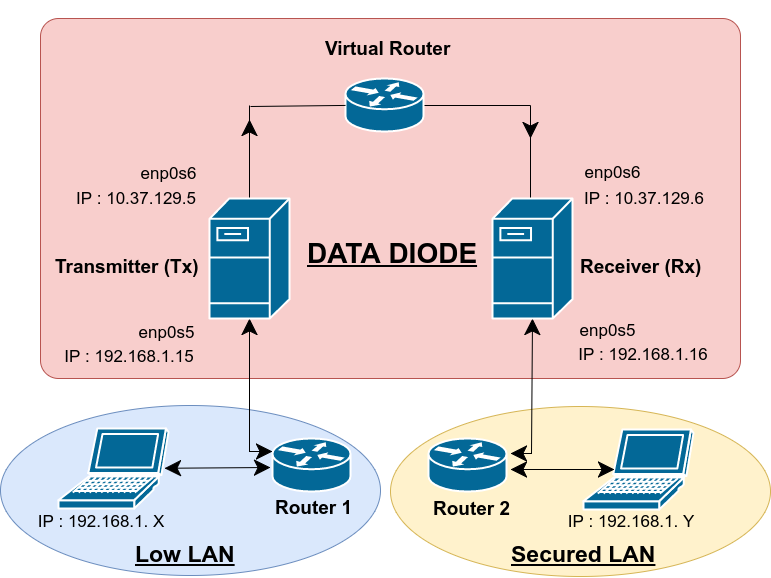
\includegraphics[scale=0.5]{images/schema2.png}
\caption{Network architecture.}
\label{fig:netvirt}
\end{figure}

As shown in Figure \ref{fig:netvirt}, within the data diode we used a virtual switch to make the connection between the transmitter and receiver. We have set up the connection by specifying for each entity a static Ipv4 address. 
\begin{enumerate}
\item[-] The transmitter (\emph{enp0s6}) Ipv4 virtual network address is : 10.37.129.5
\item[-] The receiver (\emph{enp0s6}) Ipv4 virtual network address is : 10.37.129.6
\end{enumerate}

Once the communication within the data diode was working, we decided to create a different network architecture in order to facilitate our implementation and testing process. The new network architecture made only for development and testing purpose is shown in Figure \ref{fig:netvirt}
\begin{figure}[!h]
\centering
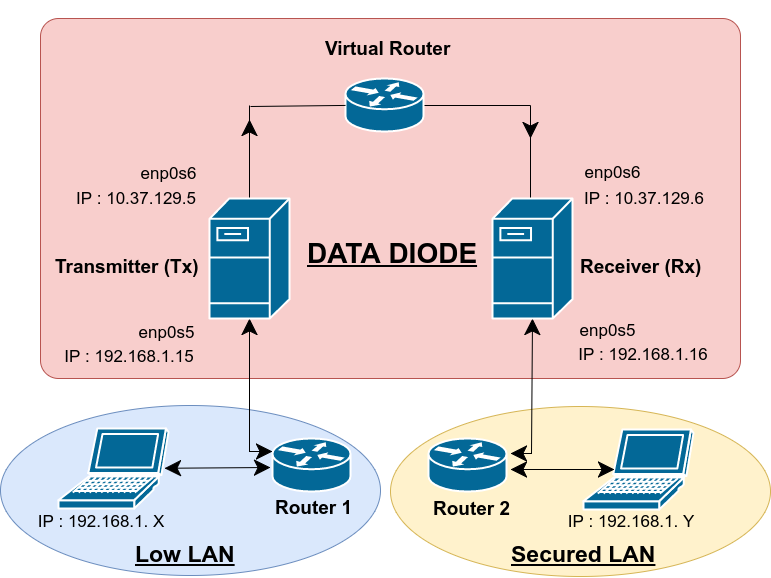
\includegraphics[scale=0.5]{images/schema2.png}
\caption{Network architecture.}
\label{fig:netvirt}
\end{figure}
We have done this to be able to communicate with the transmitter but also with the receiver from a the same computer and without needing to change networks configurations each time. We configured the outside network interface manually :
\begin{enumerate}
\item[-] The transmitter (\emph{enp0s5}) Ipv4 external network address is : 192.168.1.15
\item[-] The receiver (\emph{enp0s5}) Ipv4 external network address is : 192.168.1.16
\end{enumerate}

However, in our client's company, both the transmitter and the receiver should not be in the same LAN because if so, the data diode will be useless. We only did this here because we needed to easily test and play with our data diode prototype.
\subsubsection{Unidirectional communication}
As mentioned earlier we should have a fiber cable between the two machines of the data diode. However because of the costs involved we simulated using a virtual network. The problem is that simulating the connection means there is bi-directional communication. In order to get closer to our real scenario we used linux firewall (iptables) to block the one way back communication within the data diode. Here is how we managed to succeed it.

\paragraph{}We defined the following iptables rules on the receiver server:
\begin{enumerate}
\item INPUT -s 10.37.129.5/32 -d 10.37.129.6/32 -p tcp -j DROP
\item INPUT -s 10.37.129.5/32 -d 10.37.129.6/32 -p udp -j ACCEPT
\item INPUT -s 10.37.129.5/32 -d 10.37.129.6/32 -p icmp -j DROP
\item OUTPUT -s 10.37.129.6/32 -d 10.37.129.5/32 -j DROP
\end{enumerate}

The first three rules is to make sure that the receiver drop every packet which do not use UDP protocol as the transportation layer. The fourth is to make sure that the receiver cannot respond in any way to the transmitter

Once we have tested those rules, we saved them into a file using the command \emph{iptables-save $>$ file}. However, once the receiver server restart, the iptables are not by default persistent, this means that these rules are disappearing after a system restart. Thus, we added a command in the \emph{interfaces} file for the \emph{enp0s6} interface : \emph{pre-up iptables-restore $<$ savedFile}. This will do the trick, when the machine reboots, the iptables rules will be restored using the saved file. In this way we managed to simulate the uni-directional communication between the transmitter and the receiver within the data diode.

\subsection{Deploying an FTP protocol}
Now that we have an unidirectional communication over UDP between the two machines of the data diode, it is now time to deploy the FTP protocol presented earlier: \emph{BlindFTP}. As this is a python2 script and that python2 is already installed by default on our Linux machines, this step is quite fast.

We downloaded the \emph{BlindFTP} script on both sides of the data diode and followed these steps:
\begin{enumerate}
\item Launched the reception on the receiver side with the command : 
\begin{center}
python bftp.py -r /path/to/receptionFolder -a IPv4ReceiverAddress
\end{center}
In this command we replaced the \emph{/path/to/receptionFolder} with the default value of \emph{/home/receiver/Desktop/reception} and the \emph{IPv4ReceiverAddress} with the receiver address mentioned above which is 10.37.129.6 .

\item Once the reception has been launched, we got to the transmitter side and launched the transmission.
\begin{center}
python bftp.py -b -S /path/to/transmissionFolder -a IPv4ReceiverAddress -P secondBeforeRecheckTheFolder
\end{center}
In this command option \emph{-b} is for loop, this means that files will be send in a loop, option -P is the interval time in seconds before rechecking the transmission folder in order to see if new files have been added or deleted, we defined this by default at 5 seconds. Option \emph{-S} is the path to the transmissionFolder, we defined by default that files will be transmitted from the folder located under \emph{/home/transmission/Desktop/transmit}. And finally the \emph{-a} option is similar to the reception command.
\end{enumerate}

Once all above was done, sending a file/folder to the other side of the data diode is revealing to be an easy task. By simply copying the desired file/folder into the transmission folder from the transmitter and within 5 seconds, it will appear on the receiver side in the reception folder defined.

\subsection{Web interface of the data diode}
As we had to implement a data diode configuration web interface, we started by making some researches about how to develop a web interface in a fast and secure way. In addition, we had to find a way to integrate our python2 bftp script. We discovered the Django web framework which avers to be written in python. Moreover, Django framework already implements countermeasures against the basics vulnerabilities of the web such as XSS \footnote{Cross-Site Scripting.}, CSRF\footnote{Cross-Site Request Forgery.} and SQL injections.

In conclusion we decide to implement our web data diode interface using the Django framework.

\subsubsection{Configuration interface}
As shown earlier in this paper in Figure \ref{fig:configadminpagetrans} and in Figure \ref{fig:configadminpagereceiv}, we created a web interface which allow to change the IPv4 network address of the \emph{enp0s5} interface, remember that this is the interface facing the external network of the data diode. We managed to do this by firstly creating a symbol link of the \emph{/etc/network/interfaces} to the \emph{/home/transmitter/Desktop/DataDiode/interfaces}. We did this because the \emph{/etc/} folder could not be modified by another user unless he is root (Linux operating system). We do not want to give root permission to the Django web server which will modify the \emph{interfaces} file according to the configuration made by the administrator on the web interface. And thus in this way, the Django server can modify the file without being root.

The Django server will use the \emph{transmitter} machine user created especially for the transmitter side.

When the administrator configure the IP network address of the servers, there will always be a reboot, in order to apply changes. Despite that generally in Linux, we could only restart the networking service to apply changes, we think that our virtual machines had a driver misconfiguration because changes could not be applied in this fast way, a reboot was always applying the newest configurations.

\subsubsection{Django and bftp.py}
The only thing left was to be able to start and stop the bftp script. What we did is very simple, we used the python library \emph{os} with which we could execute bash commands. Thus, we implemented some functions to start and stop the bftp script. However this sound easy, stopping the script avers to be a difficult task. Nor Ctrl+C, nor Ctrl+D was not working. The only way to stop the script is by killing it using the \emph{kill PID} Linux command. Thus, each time we start the script we store the pid of the process and when the stopping function gets called, we execute the kill bash command.

\section{Demonstration plan}
On Friday 8th of December we are going to demonstrate our data diode prototype.
\subsection{Objectives}
The goal of the demonstration is to prove the proper functioning of the system. 
\begin{enumerate}
\item[-] We will show how users can sends file through the data diode and how they could interact with it.
\item[-] We will show how to configure the data diode, starting stopping the data diode.
\item[-] We will show how to configure network Ipv4 address of the data diode servers (transmitter and receiver). This configuration will be done for the external network of the data diode (\emph{enp0s5} interface).
\end{enumerate}

\subsection{Hardware materials}
We will use the following material in order to get closer to our real life scenario.
\begin{enumerate}
\item[-] One computer on which 2 virtual machines will be installed: the transmitter and the receiver.
\item[-] Two computers, one for communicating with the transmitter and one for the receiver.
\item[-] A router to communicate easily with both side of the data diode.
\end{enumerate}
 
\subsection{Presentation flow}
We will start with an already set up data diode prototype. Here is the step by step presentation flow that we will follow:
\begin{enumerate}
\item Starting the reception on the receiver side using the default account.
\item Authenticating using an administrator, starting the transmission.
\item Authenticating to the web interface using a normal user account and as an admin user.
\item Uploading a file and sending it through the data diode.
\item Downloading and deleting a file from both side of the data diode.
\item Changing the Ipv4 network address of both transmitter and receiver.
\end{enumerate}
 
\clearpage
\begin{thebibliography}{9}
\bibitem{data-diode-work}
DEEP SECURE,
\textit{How	Does a Data Diode Work?}
Discussion Paper, February 2017.

\bibitem{data-diode-SANS-Institute}
SANS Institute InfoSec Reading Room,
\textit{Tactical Data Diodes in Industrial Automation and Control Systems}, January 2015.

\bibitem{data-diode-transport}
CS Risk Management and Compliance Ltd,
\textit{Data Diode vs Firewall Feasibility}, September 2016. [Online]. Available: \url{https://csriskmanagement.co.uk/data-diode-vs-firewall-feasibility/} [Accessed: 30- Oct- 2017]

\bibitem{data-diode-transport}
BlindFTP,
\textit{Blind ftp protocol}[Online]. Available: \url{https://www.decalage.info/fr/python/blindftp} [Accessed: 30- Oct- 2017]

\bibitem{Livre}
David Basin AND Patrick Schaller AND Michael Schlapfer,
\textit{Applied Information Security, A hands-on Approach},
Springer.

\bibitem{data-diode-documentation}
Philippe Lagadec and Laurent Villemin,
\textit{BlindFTP documentation}
Documentation,
16 August 2010.




\end{thebibliography}
\end{document}